\documentclass[11pt,onecolumn]{article}
\usepackage[margin=1in]{geometry}
\usepackage{amsmath,amssymb}
\usepackage{graphicx}
\graphicspath{{figures/}}
\usepackage{booktabs}
\usepackage{array}
\usepackage[numbers,sort&compress]{natbib}
\usepackage{caption}
\usepackage[colorlinks=true,allcolors=blue]{hyperref}
\usepackage{changepage}

\title{Exhaustive single-layer circuit mapping of a single-cell foundation model reveals massive redundancy, heavy-tailed hub architecture, and layer-dependent steering directionality}
\author{Ihor Kendiukhov\\ Department of Computer Science, University of T\"ubingen, T\"ubingen, Germany\\ \texttt{kendiukhov@gmail.com}}
\date{}

\begin{document}
\maketitle

\begin{abstract}
Mechanistic interpretability of single-cell foundation models has relied on selective feature sampling, pairwise interaction testing, and observational trajectory analysis, with edge-calling rules never calibrated against a null. Using sparse autoencoders trained on Geneformer V2-316M residual streams, we exhaustively traced all 4{,}065 active features at layer~5 by causal ablation across 20 K562 cells, retaining the per-cell effects so that the edge criterion (Cohen's $d>0.5$, consistency $>0.7$) could be calibrated against a sign-flip permutation null. Its empirical false-discovery rate is 3.6\%, and 79\% of the 1{,}393{,}850 called edges survive false-discovery control, giving a graph of $\approx$1.1M edges; at a looser threshold ($|d|>0.3$) a third of the graph would be noise. Feature degree proves largely a restatement of activation frequency (Spearman $\rho=0.84$); the degree distribution is heavy-tailed but not scale-free (power-law exponent 6.05, indistinguishable from lognormal or exponential); and annotation does not predict computational centrality---the top-20 layer-5 hubs are 60\% annotated against a 53.8\% background ($p=0.66$), while at layers 8 and 14 hubs are significantly annotation-depleted. Three-way ablation of 12 triplets shows redundancy deepening from 0.70 (pairwise) to 0.53 (three-way), equally for triplets whose features share no pathway; superadditive targets are rare (0.087\%) and 4.9$\times$ more frequent between pathways than within them, though not significantly so. Steering an expanded panel of 80 switch features shows that layer-17 ON-switch features shift the model toward a held-out maturity probe (83\% of cells) while layer-17 OFF-switch features shift it away (88\% of cells; $p=0.0055$): directionality is encoded by the feature, not the layer. Finally, feature degree does not predict CRISPRi knockdown effect size in K562 ($\rho=0.02$): model-internal centrality and biological perturbation strength are unrelated, bounding what ablation-derived circuit maps can claim.
\end{abstract}

\paragraph{Highlights.}
\begin{itemize}
\item An uncalibrated SAE edge criterion is shown to have a 3.6\% false-discovery rate.
\item A feature's circuit degree is largely a restatement of its activation frequency.
\item The degree distribution is heavy-tailed but statistically not scale-free.
\item Steering direction is encoded by the SAE feature, not by the transformer layer.
\item Circuit centrality does not predict CRISPRi knockdown effect size in the same cells.
\end{itemize}

\noindent\textbf{Keywords:} mechanistic interpretability; sparse autoencoders; single-cell foundation models; causal circuit analysis; Geneformer; false-discovery control

\section{Introduction}
\label{sec:intro}

Single-cell foundation models such as Geneformer~\citep{theodoris2023transfer}, scGPT~\citep{cui2024scgpt}, scBERT~\citep{yang2022scbert}, and scFoundation~\citep{hao2024large} learn rich representations of cellular state from large-scale transcriptomic data~\citep{regev2017human,zheng2017massively}. Built on the transformer architecture~\citep{vaswani2017attention,devlin2019bert}, they encode genes as tokens in a high-dimensional residual stream~\citep{he2016deep,elhage2022superposition} in which biological information is distributed across many dimensions in superposition~\citep{elhage2022superposition}. Recent mechanistic-interpretability work~\citep{bereska2024mechanistic,olah2020zoom} has applied sparse autoencoders (SAEs)~\citep{cunningham2023sparse,bricken2023monosemanticity,gao2024scaling,sharkey2022taking} to decompose these representations into interpretable biological features~\citep{kendiukhov2025sae_atlas}, trace causal circuits between them~\citep{kendiukhov2025circuits}, and identify sparse feature circuits~\citep{marks2024sparse,conmy2023towards}.

Three systematic limitations constrain these analyses. First, \emph{selection by annotation:} only $\sim$30 features per layer have been traced, chosen from the most biologically annotated, so unannotated features that may serve critical computational roles are never examined. Second, \emph{pairwise-only interactions:} combinatorial ablation has tested only pairs of features, leaving open whether higher-order interactions---synergy or deeper redundancy---emerge at third or higher orders. Third, \emph{observational trajectory dynamics:} the discovery that certain features track differentiation trajectories~\citep{trapnell2014dynamics,wolf2019paga} was correlational, and no interventional evidence established that amplifying these features shifts the model's representation of cell state.

A fourth limitation cuts across all of them and, we argue, must be resolved before any of the others can be interpreted: \emph{the edge-calling criterion has never been calibrated.} Edges are retained when the ablation effect exceeds a fixed effect size ($|d|>0.5$) in a fixed fraction of cells ($>70\%$), with 20 cells per feature and no null distribution, no false-discovery control, and no sensitivity analysis. Since the graph contains $\sim$5.6$\times 10^7$ tests, even a small per-test false-positive rate would dominate the reported edge count. We therefore begin by measuring the false-discovery rate of the criterion against an empirical null.

This paper addresses all four. We calibrate edge calling against a sign-flip permutation null and report a false-discovery-controlled graph; we trace every active feature at a single source layer; we extend combinatorial ablation to three-way interactions, contrasting same-pathway, cross-pathway and random feature triplets; and we perform trajectory-guided feature steering---drawing on activation steering and representation engineering methods developed for language models~\citep{turner2023activation,li2024inference,zou2023representation}---evaluated against readouts that are independent of the signature used to select the steered features.

\paragraph{Scope and interpretation.}
Every intervention in this study is performed on the internal activations of a trained neural network. ``Ablation'' sets an SAE coefficient to zero and ``steering'' multiplies it; both are interventions on Geneformer, not on cells. Accordingly, ``causal'' throughout this paper means \emph{causal within the model}: an edge $A\to B$ asserts that setting feature $A$ to zero changes feature $B$, and nothing more. Such interventions cannot, on their own, establish biological regulation, differentiation control, or a change in the state of a real cell. We make three claims of decreasing modesty and hold each to the evidence that supports it. Model-internal claims (graph structure, redundancy, hub importance) rest on interventions and are stated as such. Representational claims (late-layer features shift the model's output toward maturation-associated genes) are tested against readouts that never see the selection signature. Biological claims are tested once, against held-out CRISPRi data, and the result of that test---a null---is reported and used to bound what the circuit map can be said to mean.


\section{Related work}
\label{sec:related}

\paragraph{Sparse-autoencoder interpretability.}
Individual residual-stream dimensions of transformer models are not interpretable in isolation: each fires for many unrelated concepts (\emph{polysemanticity}) because the model packs more concepts into the representation than it has dimensions (\emph{superposition})~\citep{elhage2022superposition,bricken2023monosemanticity}. A sparse autoencoder (SAE) re-expresses each residual vector as a sparse combination of learned directions (``features''); empirically each direction tends to fire for a single coherent program in both language~\citep{cunningham2023sparse,templeton2024scaling} and biology~\citep{kendiukhov2025sae_atlas}. Causal interventions on these features---\emph{ablation}~\citep{pearl2009causality,vig2020causal,geiger2021causal} (set the SAE coefficient to zero) and \emph{steering}~\citep{turner2023activation,li2024inference,zou2023representation} (multiply by $\alpha>1$)---are the latent-space analogues of CRISPRi knockdown and overexpression of a biological program, and let one read off circuit edges that survive a stringent ``$|d|>0.5$ in $>70\%$ of cells'' causal-consistency criterion.

\paragraph{Inputs taken from prior work, restated.}
Three artefacts are taken as inputs rather than re-derived. Because two of them are described in preprints, we restate here the exact construction and the validation each passed, so that no result below requires consulting another manuscript. All three are deposited with the code (see the Data availability statement).

\emph{(i) The layer-wise SAEs}~\citep{kendiukhov2025sae_atlas}. TopK sparse autoencoders~\citep{makhzani2013ksparse} ($k=32$, 4$\times$ overcomplete; $d_\mathrm{model}=1{,}152 \to d_\mathrm{SAE}=4{,}608$) were trained on $\sim$4.05M K562 residual-stream token positions, one SAE per layer. Selection criteria for the \emph{active} feature set used throughout: activation frequency $\geq 0.001$, which at layer~5 retains 4{,}065 of 4{,}608 features. Validation: a monosemanticity audit (top-gene/ontology-term Jaccard $\bar J = 0.034$ versus a matched random-pair baseline of $0.0023$, a 14.6$\times$ enrichment) and cross-context stability of top-50 gene loadings against an independently trained Tabula Sapiens SAE (mean Jaccard $0.13$ over 39 Hungarian-matched pairs at decoder cosine $>0.3$); both are reproduced in the Supplementary Material.

\emph{(ii) The selective circuit map}~\citep{kendiukhov2025circuits}. Thirty features per layer were traced by pairwise causal ablation across 200 cells. The selection rule was an \emph{annotation-quality score}: the number of significant ontology enrichments (GO~BP, KEGG, Reactome, STRING, TRRUST) weighted by $-\log_{10}(p)$, taking the top 30. That trace produced 52{,}116 significant L5 edges under the same $|d|>0.5$, consistency $>0.7$ criterion, and a median pairwise redundancy ratio of $0.74$ with no superadditive targets across 20 same-pathway pairs. It is used here only as the comparison point in Table~\ref{tab:selective_vs_exhaustive}; its edge count inherits the calibration problem quantified below.

\emph{(iii) The differentiation-tracking (``switch'') features}~\citep{kendiukhov2025circuits}. Fourteen features (5/2/4/3 at L0/L5/L11/L17) were reported as tracking pseudotime in Tabula Sapiens immune cells. The published panel mixed two selection rules and its reported effect sizes are not reproducible from a single one, so this study does not rely on it. We re-derive the panel from the deposited 481-cell SAE activation matrices under one stated rule (Materials and methods); the resulting panel is a strict superset that contains all 14 published features. Because the original analysis was observational, it could not distinguish ``encodes differentiation'' from ``correlates with differentiation.'' A companion study~\citep{kendiukhov2025systematic} further showed that attention-based interpretability captures co-expression rather than causal regulation.

\paragraph{Glossary of recurring terms.}
For brevity we use throughout:
\emph{residual stream}---the additively-accumulating per-gene vector at a given transformer layer;
\emph{feature}---one column of the SAE decoder, $d_f \in \mathbb{R}^{1152}$;
\emph{activation frequency}---fraction of tokens on which $f$ has non-zero coefficient;
\emph{degree}---number of significant outgoing edges of a feature, summed over the measured downstream layers;
\emph{hub feature}---a feature in the top 1.8\% of its source layer by degree;
\emph{switch feature}---a feature whose activation differs between early- and late-pseudotime immune cells by Cohen's $d\geq 0.5$ (ON-switch) or $\leq -0.5$ (OFF-switch), defined operationally in the Materials and methods section;
\emph{redundancy ratio} $R_n = |d_{A_1\cup\dots\cup A_n}| / \sum_i |d_{A_i}|$, where $R<0.8$ is subadditive, $0.8\leq R\leq 1.2$ additive, and $R>1.2$ superadditive;
\emph{state shift} $\Delta s$---change in cosine-similarity-difference of the cell's logits toward the late vs.\ early gene signature, defined in the Materials and methods section;
\emph{fraction positive}---fraction of steered cells for which a given readout increases.


\paragraph{Scope of the present study.}
The experiments below move beyond the prior results in four directions: (i)~calibration of the edge-calling criterion against an empirical null, which fixes the meaning of every edge count reported here or previously; (ii)~exhaustive tracing of all 4{,}065 active features at L5 rather than 30 selected features---a 135-fold increase in feature coverage, purchased at a tenfold reduction in cells per feature; (iii)~three-way rather than pairwise combinatorial ablation, with cross-pathway and random triplets as contrasts; and (iv)~steering of an expanded switch-feature panel that includes OFF-switch features as a directional control, with dose--response and three readouts independent of the selection signature. Atlas-level statistics are treated as inputs and not re-derived. ``Exhaustive'' refers throughout to feature coverage at one source layer, not to the model: a single source layer samples $1/18$ of Geneformer's depth, one cell line, one SAE training context, and one model.


\section{Materials and methods}
\label{sec:methods}

\subsection{Model and sparse autoencoders}

All experiments used Geneformer V2-316M~\citep{theodoris2023transfer}, an 18-layer, 18-head transformer pre-trained on $\sim$100\,M single-cell transcriptomes. TopK SAEs~\citep{makhzani2013ksparse} ($k=32$, 4$\times$ overcomplete) were trained on residual-stream activations at each layer from 4.05M K562 token positions as described in~\citep{kendiukhov2025sae_atlas}; we use these existing layer-wise SAEs without retraining. Checkpoint hashes, seeds, software versions, and a script-to-artefact map for every number in this paper are given in \texttt{REPRODUCIBILITY.md} in the code release.

\subsection{Feature annotation pipeline}
\label{sec:annotation}

Each SAE feature was assigned a biological label by the following pipeline; the same pipeline is used in every subsequent results subsection.
(1)~For every active feature $f$ at layer $\ell$, we collect (gene-token, activation-coefficient) pairs over $\sim$4\,M K562 token positions; per gene $g$ we record its mean activation of $f$ (\emph{mean\_activation}$_g$) and fire-count.
(2)~The \emph{top-gene set} $T_f$ is the top 50 genes by mean\_activation, restricted to genes with fire-count $\geq 5$.
(3)~$T_f$ is tested against every GO biological process~\citep{ashburner2000go}, KEGG~\citep{kanehisa2000kegg}, and Reactome~\citep{jassal2020reactome} term using Fisher's exact test (one-sided), with background equal to the union of top-gene sets across all features at $\ell$. Term sizes are clipped to $[5, 500]$ genes.
(4)~Benjamini--Hochberg correction~\citep{benjamini1995controlling} is applied across all (feature, term) tests; a feature receives the term with smallest $q$-value satisfying $q<0.05$, or is labelled \emph{unannotated}.
We validate this pipeline in three complementary ways in the Supplementary Material: (a)~null calibration on $10^3$ random size-50 gene sets yields empirical FPR $=$\,$\mathbf{1.0\%}$; (b)~recall against 29 canonical K562-active processes drawn from GO/KEGG/Reactome; (c)~cross-context stability of top-50 gene loadings between the K562-trained SAE and an independently-trained Tabula Sapiens SAE.

\subsection{Exhaustive circuit tracing}

\paragraph{Source and downstream layers.}
We chose layer~5 as the exhaustive-tracing source for three reasons grounded in the SAE atlas~\citep{kendiukhov2025sae_atlas}. (i)~At L0--L3 the per-layer annotation rate is dominated by raw-expression features (housekeeping, ribosomal, mitochondrial); at L11+ a growing fraction of features encode global cell-type identity rather than pathways. L5 is where \emph{pathway-level features} are best resolved. (ii)~The prior selective circuit map~\citep{kendiukhov2025circuits} used L5 as its primary source layer, so tracing exhaustively at L5 enables a direct head-to-head comparison (Table~\ref{tab:selective_vs_exhaustive}). (iii)~The qualitative result is not specific to L5: a 500-feature subsample of the same protocol at L2, L8, and L14 replicates each finding (Results, ``Annotation status does not predict centrality''). We chose downstream layers $\{6, 11, 17\}$ as adjacent, middle, and final readouts; the qualitative attenuation curve is preserved when all 12 downstream layers are measured for the top 200 hubs (Supplementary Material).

\paragraph{Protocol.}
For each of the 4{,}065 active features at layer~5, we performed causal ablation tracing~\citep{pearl2009causality,vig2020causal,geiger2021causal} across 20 randomly sampled K562 cells. A clean forward-pass cache was pre-computed once, storing source-layer hidden states, SAE encodings, and downstream clean SAE activations for all cells. For each feature we set its TopK coefficient to zero in the source-layer residual stream, injected the modified stream into the next encoder layer, propagated through the remaining layers, and encoded the downstream hidden states through the corresponding SAEs. Writing $\delta_{f\to t}^{(c)}$ for the change in the activation of downstream feature $t$ in cell $c$ (averaged over the token positions at which $f$ fires), the effect size is the one-sample statistic $d = \overline{\delta}/\mathrm{SD}(\delta)$ over the $n$ cells in which $f$ fires, and the \emph{consistency} is $\max(n_+, n-n_+)/n$ with $n_+$ the number of cells with $\delta>0$. Because $n=20$, we correct $d$ for small-sample bias, reporting Hedges' $g = d\,(1 - 3/(4n-5))$~\citep{hedges1981distribution}.

\paragraph{Edge calling and its calibration.}
\label{sec:calibration}
The published criterion retains an edge when $|d|>0.5$ and consistency $>0.7$. Applied to $4{,}065\times 4{,}608\times 3$ tests, this needs a null. Note first that the model is deterministic, so a downstream feature that lies on no path from $f$ has $\delta^{(c)}=0$ in every cell; the relevant null is therefore not ``no perturbation'' but ``no \emph{consistently directed} effect''. We test exactly that with a sign-flip permutation~\citep{good2000permutation}: for each (source, target, downstream layer) we flip the sign of each cell's $\delta^{(c)}$ independently, $B=500$ times, and recompute $d$ and consistency. This null is conditioned on the observed effect magnitudes, and targets with identically zero $\delta$ remain zero and can never generate a null edge. Three quantities follow. (i)~The \emph{empirical false-discovery rate} is the mean number of null edges divided by the observed number. (ii)~A permutation $p$-value per target, $p = (1 + \#\{|d_{\text{perm}}| \geq |d_{\text{obs}}|\})/(1+B)$, computed over every \emph{live} target (one whose $\delta$ is not identically zero) and corrected across the whole family by Benjamini--Hochberg~\citep{benjamini1995controlling}. The \emph{calibrated} edge set requires $q<0.05$ \emph{and} $|g|>0.5$ \emph{and} consistency $>0.7$. (iii)~A threshold sweep over $|d|\in\{0.3,0.5,0.8,1.0,1.5,2.0\}\times$ consistency $\in\{0.6,\dots,1.0\}$, reporting for each cell of the grid the edge count, the expected null count, and the Spearman correlation of the induced hub ranking with the default. Permutation analysis is run on a 600-feature subset comprising the 200 highest-degree features (so the hub table is exact) plus a degree-stratified sample of 400; the calibrated graph size for all features is obtained by applying each degree decile's survival ratio to the features in that decile.

A second, orthogonal null asks whether an edge reflects the \emph{identity} of the ablated feature rather than the magnitude of the displacement it causes. For 200 features stratified by degree we replaced the ablation displacement $\Delta h = \mathrm{dec}(h_{f=0}) - \mathrm{dec}(h)$ by a random Gaussian direction rescaled to the same per-position norm, and repeated the measurement (Supplementary Material).

\paragraph{Sample size.}
The choice of $n=20$ cells per feature is a coverage--sensitivity trade-off against the $n=200$, 30-feature selective baseline, not an increase in power. The Supplementary Material characterises it directly by re-running the L5 trace on 48 features stratified by edge-count quartile at $n\in\{5,10,20,40,80,160\}$: mean edges per feature \emph{falls} monotonically with $n$ (472 at $n=5$ to 187 at $n=160$), because a larger $n$ tightens $\mathrm{SD}(\delta)$ and so raises the bar to pass $|d|>0.5$; test--retest correlation at $n=20$ is $r=0.91$. Edge counts from runs with different $n$ are therefore not comparable, and we never compare them without saying so.

\subsection{Higher-order combinatorial ablation}

Feature triplets were constructed with one feature at each of layers 0, 5 and 11, in three classes: \emph{same-pathway} (all three annotated to one pathway), \emph{cross-pathway} (three different pathways), and \emph{random} (drawn at random from features with activation frequency $\geq 0.02$, matched in frequency to the other two classes, and rejected if any two picks shared a pathway). Pathways were assigned to annotation strings by an ordered keyword map (Supplementary Material); the ordering places DNA-damage terms before metabolism so that, for example, \emph{DNA Metabolic Process} is not filed as metabolism. For each triplet, 7 ablation conditions (A, B, C, AB, AC, BC, ABC) were tested on 100 K562 cells, measuring at layer~17. Features are ablated sequentially along the forward pass, each re-encoded on the already-perturbed residual stream.

Over targets significant in at least one condition, the three-way redundancy ratio is $R_{ABC}=|d_{ABC}|/(|d_A|+|d_B|+|d_C|)$ and the higher-order interaction term is $I_{ABC}=|d_{ABC}|-|d_{AB}|-|d_{AC}|-|d_{BC}|+|d_A|+|d_B|+|d_C|$. A target is \emph{subadditive} if $R<0.8$, \emph{additive} if $0.8\leq R\leq 1.2$, and \emph{superadditive} if $R>1.2$; we retain these thresholds from the pairwise study so that orders are comparable. Confidence intervals on the median $R_{ABC}$ and $I_{ABC}$ are percentile bootstrap intervals over targets (1{,}000 resamples), targets being the unit the median is taken over; the superadditive rate per triplet is given a Wilson interval. Superadditive rates between triplet classes are compared by Fisher's exact test. We report the 12 triplets run under this protocol together with the 8 previously reported at 200 cells per condition.

\subsection{Trajectory-guided feature steering}
\label{sec:steering_methods}

\paragraph{Feature panel.}
Switch features are re-derived from the 481 Tabula Sapiens~\citep{tabula2022tabula} immune cells and their cached per-cell SAE activations at layers 0, 5, 11 and 17. Cells are split at the terciles of diffusion pseudotime~\citep{haghverdi2016diffusion}; for each feature with activation frequency $\geq 0.05$ we compute Cohen's $d$ between the late and early terciles with pooled standard deviation. The panel is the top 12 \emph{ON-switch} features ($d\geq 0.5$; higher in mature cells) and the top 8 \emph{OFF-switch} features ($d\leq -0.5$) at each of the four layers: 80 features in total. All 14 features of the previously published panel fall inside this set.

The OFF-switch features are a directional control. If ``late-layer features push cells toward maturity'' were a property of the layer or of the metric, OFF-switch features at that layer would push in the same direction as ON-switch features; if directionality is carried by what the feature encodes, they will push the opposite way.

\paragraph{Intervention.}
Steering followed the activation-addition framework~\citep{turner2023activation,li2024inference}, multiplying the feature's SAE coefficient by $\alpha\in\{1.5, 2, 3, 5, 8\}$ (the full grid for the top 4 features per layer per direction, i.e.\ 32 features; $\alpha\in\{2,5\}$ for the rest) and reconstructing the residual stream as $h'_\ell = h_\ell + (\alpha-1)\cdot a_f\cdot d_f$, where $a_f$ is the activation coefficient and $d_f$ the decoder direction. Interventions are applied in the 160 early-pseudotime cells (bottom tercile) in which the feature fires. Features active in fewer than 10 such cells are excluded from all reported statistics (5 of 80, of which 3 belong to the dose-response grid, leaving 29 there).

\paragraph{Readouts.}
The published readout is the \emph{state shift}
\[
\Delta s = \cos(z', g_\text{late}) - \cos(z', g_\text{early}) - [\cos(z, g_\text{late}) - \cos(z, g_\text{early})],
\]
with $z, z'$ the clean and steered mean logit vectors over gene positions, and $g_\text{late}, g_\text{early}$ the mean logit profiles of the late and early pseudotime terciles. This metric is built from the same pseudotime embedding used to select the features, so it cannot by itself establish that steering moves the model along a differentiation axis. We therefore add three readouts that never see the pseudotime signature:
\begin{enumerate}
\item \emph{Marker score.} The change in mean output logit over a literature-defined terminal-maturation gene panel minus the change over a progenitor panel (18 genes each; listed in the Supplementary Material).
\item \emph{$\Delta P(\text{terminal})$.} A logistic probe on Geneformer's mean-pooled final-layer embedding, trained on up to 1{,}500 Tabula Sapiens hematopoietic cells \emph{disjoint} from the 481 steered cells, with labels taken from the cell-type ontology (immature: haematopoietic stem cell, haematopoietic precursor, common myeloid progenitor, naive CD4/CD8 T cell; terminal: neutrophil, macrophage, plasma cell, mature NK T cell, granulocyte, basophil). Five-fold cross-validated AUC $=0.838\pm0.032$.
\item \emph{$\Delta$ predicted pseudotime.} A ridge probe from clean embeddings to diffusion pseudotime, fit on the 321 non-steered cells (five-fold cross-validated $R^2=0.33$) and applied to the steered embeddings. Steering acts in latent space, so diffusion pseudotime cannot literally be recomputed from a steered expression profile; this learned map is the operational substitute, and we label it as such.
\end{enumerate}
For each readout we report the per-feature mean, the fraction of cells with a positive change, a one-sample $t$-test on the per-cell values with Benjamini--Hochberg correction across the panel, and the Spearman correlation between the effect magnitude and $\alpha$ (dose--response). ON- and OFF-switch features are compared per layer by the Mann--Whitney $U$ test. $\Delta s$ is additionally recomputed under signatures derived from bone-marrow cells only and from blood plus spleen cells only, to test whether its sign transfers across tissue.

\paragraph{State-shift null baselines.}
The primary directional controls for the expanded panel are the OFF-switch contrast and the held-out readouts above. As additional support that the state-shift signal exceeds chance, the state-shift metric $\Delta s$ was also benchmarked against three null distributions and a ceiling intervention: (a) a \emph{random-feature null}---the identical protocol applied to 210 non-switch features (32/54/67/57 at L0/5/11/17); (b) a \emph{random-direction null}---$d_f$ replaced with a unit Gaussian direction; (c) a \emph{sign-shuffled null}---the sign of $(\alpha-1)$ flipped for half the cells per feature; and a \emph{ceiling intervention} that steers along the residual-stream projection of $(g_\text{late}-g_\text{early})$ to bound the maximum $\Delta s$ achievable under any single-direction perturbation. Protocols and results are in the Supplementary Material.

\subsection{Model-internal importance of hub features}

To test whether high-degree features matter to the model, we ablated single features and measured the damage to Geneformer's masked-gene prediction on 50 held-out K562 cells with 15\% of gene tokens masked (mask positions drawn once and reused across all arms). Three arms of 50 features each: the 50 highest-degree L5 features; 50 randomly drawn non-hub features; and 50 non-hub features matched one-to-one to the hubs on log activation frequency. The frequency-matched arm is necessary because degree and activation frequency are strongly coupled (Results); without it the comparison would only rediscover that frequently firing features matter. We report the change in masked-token cross-entropy and in top-1 recovery accuracy.

\subsection{Generalisation across SAE training context}

To separate ``the hub architecture is specific to K562'' from ``the K562-trained feature basis does not transfer'', we repeated the tracing protocol on Tabula Sapiens immune cells using SAEs trained natively on Tabula Sapiens activations, which exist at layers 0, 5, 11 and 17. Source layer 5, downstream layers $\{11, 17\}$, 400 randomly sampled active features, 20 cells. The K562 trace is restricted to the same two downstream layers for a like-for-like comparison of the degree distribution, its skewness and Gini coefficient, the top-20 unannotated fraction, and the degree--frequency coupling.

\subsection{Biological grounding against CRISPRi ground truth}

Interventions on SAE coefficients are interventions on a model. To ask whether the resulting graph carries information about biology, we tested a prediction it makes: genes loading on high-degree features should be genes whose knockdown perturbs the K562 transcriptome strongly. From the genome-scale K562 CRISPRi screen~\citep{replogle2022mapping} we computed, for each of 2{,}023 perturbed genes with $\geq 20$ cells, the Euclidean distance between its pseudobulk profile and the non-targeting control profile in log-normalised space, standardised against a control-resampling null matched on cell count, giving a shift $z$-score. Each L5 feature received a \emph{perturbation strength} equal to the mean $z$ of those of its top-50 loading genes present in the screen (2{,}384 features had $\geq 5$). We report the Spearman correlation between feature degree and perturbation strength, its partial correlation given activation frequency and mean expression, a gene-label permutation null (500 permutations), and a hub-versus-non-hub comparison.

\section{Results}
\label{sec:results}

\subsection{Edge calling, calibrated against an empirical null}

Every edge count in this literature---1{,}393{,}850 here, 52{,}116 in the selective map---is the output of a fixed decision rule ($|d|>0.5$, consistency $>0.7$) applied without a null. We therefore calibrated the rule before using it.

Since Geneformer is deterministic, a downstream feature that lies on no path from the ablated feature has an exactly zero effect in every cell: 56.8\% of the tested (source, target, downstream-layer) triples are of this kind and can never yield an edge. The live tests are those with a non-zero effect, and for them the relevant null hypothesis is that the effect has no consistent direction across cells. Flipping the sign of each cell's effect independently ($B=500$ permutations) gives the distribution of $d$ and consistency under that hypothesis, conditioned on the observed magnitudes.

On the 600-feature calibration subset (the 200 highest-degree features plus a degree-stratified sample of 400), the criterion produced 327{,}609 edges against an expected 11{,}915 under the null: an \textbf{empirical false-discovery rate of 3.6\%}. Requiring in addition that each edge survive Benjamini--Hochberg control at $q<0.05$ across the 3.59M live tests retains 86.2\% of them. Extrapolating each degree decile's survival ratio to the whole feature set gives a calibrated graph of \textbf{$\approx$1{,}104{,}000 edges}, 79.2\% of the 1{,}393{,}850 called by the uncalibrated rule, with a mean of 272 edges per feature.

The criterion is far more conservative than its ingredients suggest. Two facts make it so: most target features are degenerate, as noted above, and among the live tests an effect that keeps the same sign in at least 15 of 20 cells \emph{and} exceeds half a standard deviation is genuinely hard to produce by chance. The threshold sweep (Supplementary Material) shows why $|d|>0.5$ matters: at $|d|>0.3$ the empirical FDR is 35.0\%, whereas at $|d|>0.5$ it is 3.6\%. Loosening the threshold to $0.3$ would multiply the edge count by 3.3 and spend a third of it on noise. Within the whole region of the grid that keeps the FDR below 5\%, the \emph{hub ranking} is essentially fixed (Spearman $\rho\geq0.91$ against the default ranking, and at least 15 of the top-20 hubs preserved), so the structural claims below do not depend on where in that region the threshold sits. Applying false-discovery control likewise leaves the hub set intact: 19 of the 20 highest-degree features are unchanged, the calibrated and uncalibrated degrees correlate at $\rho=0.99$, and the top-20 still contains 8 unannotated features.

A second null asks not whether an edge could arise from directionless noise but whether it reflects the \emph{identity} of the ablated feature rather than the size of the displacement its removal causes. For 200 features stratified by degree we replaced each ablation displacement with a Gaussian random direction of the same per-position norm. Real ablations produce 15.7 times as many edges as norm-matched random directions (mean 356 versus 23 per feature; Wilcoxon signed-rank $p=2\times10^{-34}$), so 94\% of the graph is attributable to which feature is removed, not merely to perturbing the residual stream by that much. The residual random-direction edges are themselves weakly degree-dependent ($\rho=0.42$), consistent with high-degree features occupying higher-variance directions.

All edge counts below use the calibrated criterion, and effect sizes are reported as Hedges' $g$.

\subsection{The layer-5 circuit map, and what coverage costs}

We traced all 4{,}065 active L5 features (activation frequency $\geq 0.001$), measuring effects at layers 6, 11 and 17 across 20 K562 cells~\citep{replogle2022mapping}. Under the calibrated criterion the graph contains $\approx$1{,}104{,}000 edges, against 1{,}393{,}850 before false-discovery control. Mean degree is 272 calibrated and 343 uncalibrated; the uncalibrated distribution has median 284 and range 0--2{,}138, with 8 features receiving no edges at all.

The comparison with selective tracing (Table~\ref{tab:selective_vs_exhaustive}) is a coverage--sensitivity trade-off, not an improvement in either direction. Exhaustive tracing sees 135$\times$ more features but uses a tenth as many cells per feature, and mean edges per feature accordingly falls from 1{,}737 to 343. As the power analysis in the Supplementary Material shows, edges per feature decreases monotonically with the number of cells (472 at $n=5$; 187 at $n=160$) because larger samples tighten $\mathrm{SD}(\delta)$ and raise the bar to pass $|d|>0.5$. The two graphs therefore answer different questions, and the total-edge ratio between them is not a measure of how much circuitry either recovers.

Causal effects attenuate monotonically with distance from the source: layer~6 received 49.8\% of edges, layer~11 31.8\%, and layer~17 18.4\% (Fig.~\ref{fig:circuit_overview}C). Measuring all 12 downstream layers for the top-200 hubs reproduces the shape (Supplementary Material), with an L6$\to$L17 attenuation ratio of 2.6 against 2.7 in the main trace.


\begin{table}[t!]
\centering
\caption{{\bf Selective versus exhaustive tracing at layer~5.} The two runs differ in feature coverage and in cells per feature, and their edge counts are therefore not directly comparable: the effect-size criterion becomes harder to pass as the number of cells grows. Calibrated counts apply the permutation-based false-discovery control.}
\label{tab:selective_vs_exhaustive}
\small
\begin{tabular}{lrr}
\toprule
Metric & Selective & Exhaustive \\
\midrule
Features traced & 30 & 4{,}065 \\
Cells per feature & 200 & 20 \\
Downstream layers & 12 & 3 \\
\midrule
Total edges (uncalibrated) & 52{,}116 & 1{,}393{,}850 \\
Total edges (FDR-controlled) & --- & $\approx$1{,}104{,}000 \\
Mean edges/feature (uncalibrated) & 1{,}737 & 343 \\
Mean edges/feature (FDR-controlled) & --- & 272 \\
Median edges/feature & --- & 284 \\
Max edges & --- & 2{,}138 \\
Features with 0 edges & --- & 8 \\
Empirical FDR at $|d|>0.5$, cons.\ $>0.7$ & --- & 3.6\% \\
\bottomrule
\end{tabular}
\end{table}

\begin{figure}[t!]
\centering
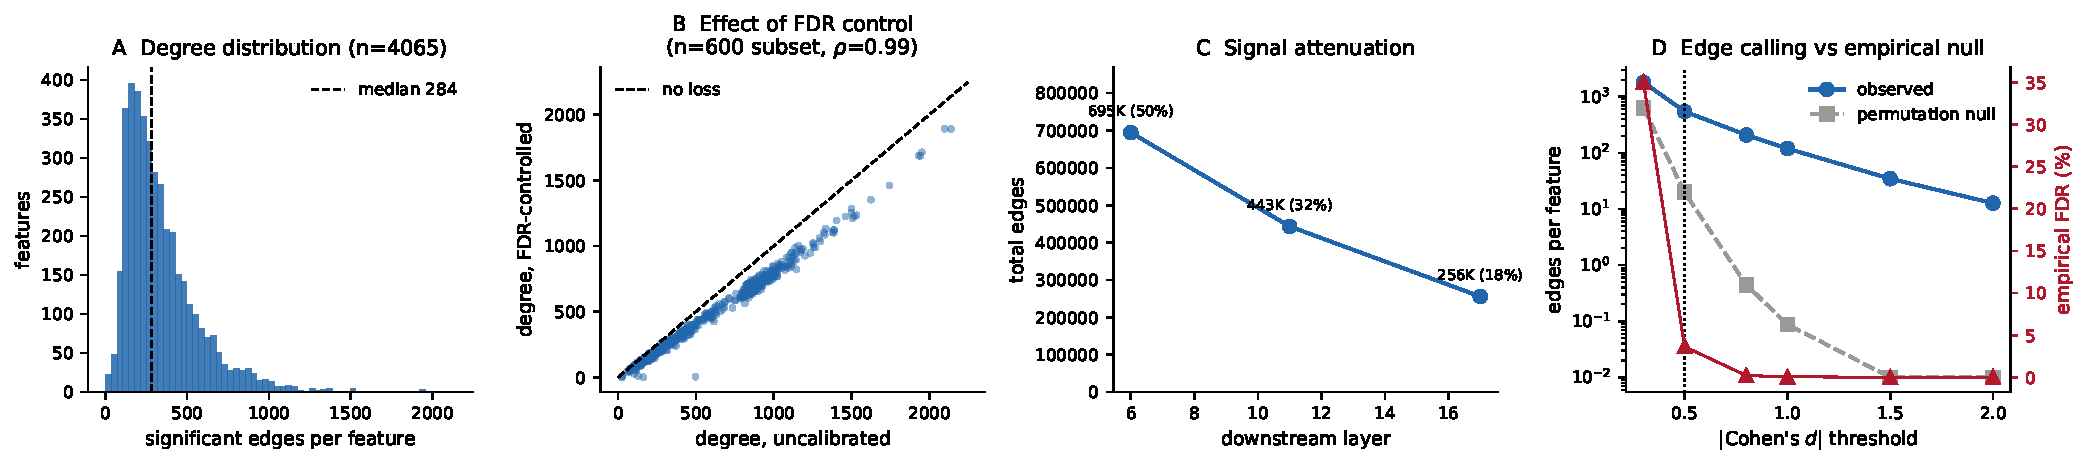
\includegraphics[width=\textwidth]{Fig1.pdf}
\caption{{\bf The calibrated layer-5 circuit map.} (A)~Degree distribution across all 4{,}065 active features. (B)~Degree before and after false-discovery control, on the 600-feature calibration subset; the ranking is preserved (Spearman $\rho=0.99$) and about a fifth of the edges are removed. (C)~Signal attenuation across downstream layers. (D)~Observed edges per feature and the sign-flip permutation null as a function of the effect-size threshold, with the resulting empirical false-discovery rate (right axis). The dotted line marks the criterion used throughout; at $|d|>0.3$ a third of the edges are noise.}
\label{fig:circuit_overview}
\end{figure}

\subsection{The degree distribution is heavy-tailed, but not scale-free}

The degree distribution is strongly right-skewed (Fig.~\ref{fig:circuit_overview}A): 72 features (1.8\%) carry more than 1{,}000 edges before false-discovery control, and 26 (0.64\%) after it. Earlier work described this as ``reminiscent of scale-free architectures''. Formal fitting does not support that description. Following \citet{clauset2009powerlaw}, a discrete power law fitted by maximum likelihood with $x_\mathrm{min}$ chosen by Kolmogorov--Smirnov minimisation gives $\alpha=6.05$ with $x_\mathrm{min}=860$, retaining only 157 of 4{,}057 features in the fitted tail. The fit is not rejected (parametric-bootstrap $p=0.95$), but neither is any alternative: likelihood-ratio tests against lognormal ($z=-0.09$, $p=0.93$), exponential ($z=+1.21$, $p=0.23$), stretched exponential ($z=+0.25$, $p=0.80$) and truncated power law ($z=-0.23$, $p=0.82$) are all inconclusive~\citep{vuong1989likelihood}. With 157 points in the tail the data cannot discriminate among these families, and an exponent of 6 lies far outside the $2<\alpha<3$ regime in which scale-free behaviour has its usual consequences. We therefore describe the distribution as heavy-tailed and hub-dominated, and make no scale-free claim---consistent with the broader finding that scale-free structure is rare in empirical networks once tested rather than asserted~\citep{broido2019scalefree}.

\subsection{Degree tracks how often a feature fires}

Before interpreting hubs biologically, one confound must be removed. A feature that fires on more token positions yields a less noisy per-cell mean effect and therefore passes the effect-size threshold on more targets. Empirically the coupling is strong: Spearman $\rho=0.84$ between activation frequency and degree ($p<10^{-300}$), and a quadratic fit in log-frequency explains 56.2\% of the variance in log-degree. The same coupling holds at every other source layer tested ($\rho=0.85$, $0.85$, $0.88$ at L2, L8, L14). ``Hub'' therefore means, to a first approximation, ``frequently active''. We report both the raw degree ranking and one residualised on log-frequency wherever the distinction matters.

\subsection{Annotation status does not predict computational centrality}

Of the 20 highest-degree L5 features, 8 are unannotated (Table~\ref{tab:top20_hubs}; Fig.~\ref{fig:hub_architecture}A,B). Against the 53.8\% annotation rate of all 4{,}065 active features, this is not a depletion of annotation among hubs---it is a slight, non-significant enrichment (60.0\% annotated among the top 20; Fisher's exact odds ratio $1.29$, $p=0.66$). The top-100 and top-1\% hubs are likewise indistinguishable from background (OR $0.82$, $p=0.36$; OR $0.67$, $p=0.21$). Across all features the association between degree and annotation is positive, weak, and driven by frequency: $\rho=+0.16$ ($p=2\times10^{-24}$) unadjusted, but $\rho=-0.04$ once activation frequency is partialled out. Ranking features by frequency-residualised degree leaves the top-20 65\% annotated (OR $1.60$, $p=0.37$; Fig.~\ref{fig:hub_architecture}C,D).

The picture changes with depth. Repeating the protocol on 500 randomly sampled features at layers 2, 8 and 14 (Table~\ref{tab:layers}), the unannotated fraction among the top-20 hubs rises from 40\% (L5) to 55\% (L2), 75\% (L8) and 80\% (L14). At L8 and L14 this \emph{is} a significant depletion of annotation among hubs (OR $0.32$, $p=0.037$; OR $0.22$, $p=0.0050$), and at L14 it survives comparison against a frequency-matched background ($p=0.038$). Deep layers concentrate their highest-degree computation in features that current ontologies do not describe.

Two conclusions follow, and only two. Annotation status carries almost no information about a feature's centrality, at any layer. And a pipeline that selects features by annotation---as the selective circuit map did---never examines 8 of the 20 highest-degree features at L5, or 16 of 20 at L14, not because hubs are preferentially unannotated but because centrality and annotation are close to independent. The methodological hazard is real; the ``annotation bias in hubs'' that would explain it is not.

\begin{table}[t!]
\centering
\caption{{\bf Hub annotation across source layers.} Top-20 unannotated fraction, and Fisher's exact test of annotation among the top-20 hubs against all traced features at that layer. L5 is the exhaustive trace; L2/L8/L14 are 500-feature random subsamples of the identical protocol.}
\label{tab:layers}
\small
\begin{tabular}{lrrrrr}
\toprule
Source & Features & Annotation & Top-20 & Odds & $p$ \\
layer & traced & rate & unannotated & ratio & \\
\midrule
L2  & 500 & 60.2\% & 11/20 (55\%) & 0.53 & 0.17 \\
\textbf{L5} & \textbf{4{,}065} & \textbf{53.8\%} & \textbf{8/20 (40\%)} & \textbf{1.29} & \textbf{0.66} \\
L8  & 500 & 50.0\% & 15/20 (75\%) & 0.32 & 0.037 \\
L14 & 500 & 51.8\% & 16/20 (80\%) & 0.22 & 0.0050 \\
\bottomrule
\end{tabular}
\end{table}


\begin{figure}[t!]
\centering
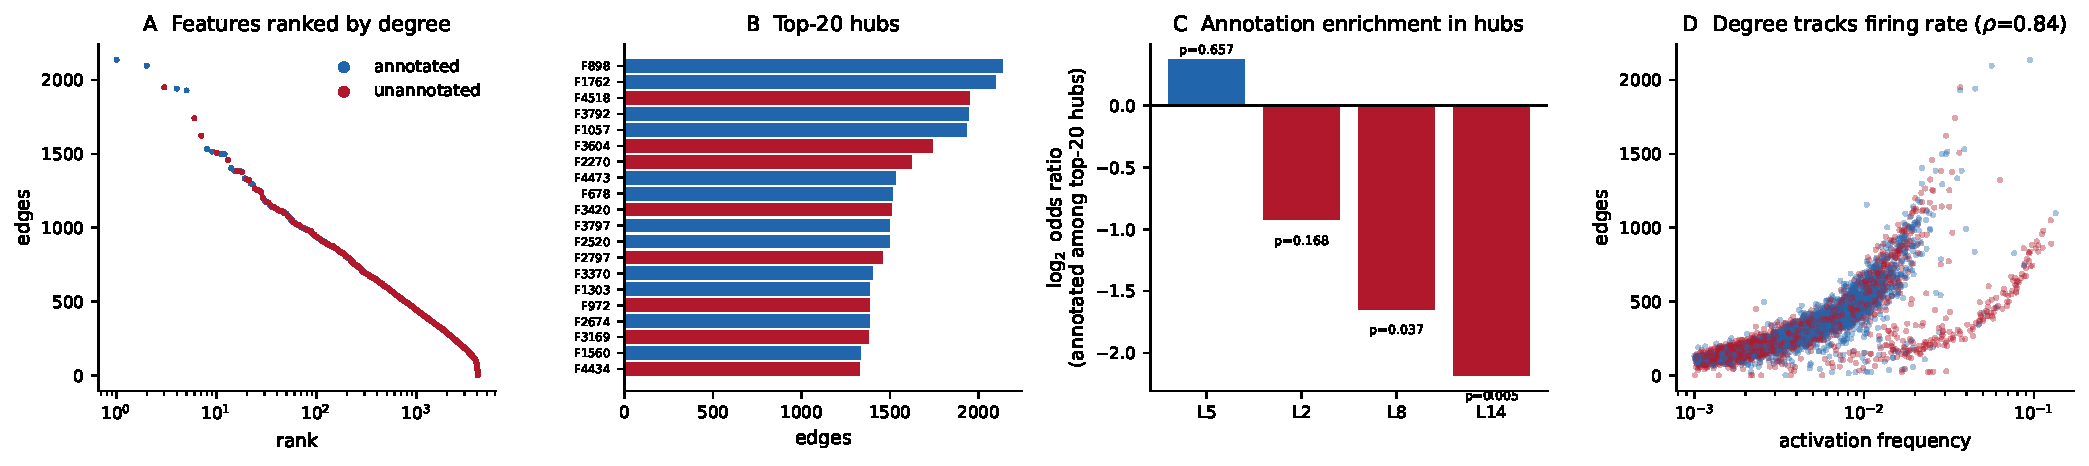
\includegraphics[width=\textwidth]{Fig2.pdf}
\caption{{\bf Hub architecture, annotation, and the frequency confound.} (A)~Features ranked by degree, coloured by annotation status. (B)~The 20 highest-degree features; red bars are unannotated. (C)~Fisher's exact odds ratio for annotation among the top-20 hubs, per source layer; values above zero indicate enrichment. Annotation is not depleted among L5 hubs, and is significantly depleted only at L8 and L14. (D)~Degree against activation frequency: a feature's degree is largely a restatement of how often it fires.}
\label{fig:hub_architecture}
\end{figure}

\begin{table}[t!]
\centering
\caption{{\bf Top 20 layer-5 hubs by degree.} Eight are unannotated. Against the 53.8\% background annotation rate this is a non-significant enrichment of annotation, not a depletion (Fisher's exact OR $=1.29$, $p=0.66$).}
\label{tab:top20_hubs}
\small
\begin{tabular}{rlrl}
\toprule
Rank & Feature & Edges & Annotation \\
\midrule
1 & F898 & 2{,}138 & Neg.\ Reg.\ Gene Expression \\
2 & F1762 & 2{,}098 & G2/M Transition \\
3 & F4518 & 1{,}951 & \textit{unannotated} \\
4 & F3792 & 1{,}943 & Transcription factors \\
5 & F1057 & 1{,}930 & Herpes simplex infection \\
6 & F3604 & 1{,}743 & \textit{unannotated} \\
7 & F2270 & 1{,}624 & \textit{unannotated} \\
8 & F4473 & 1{,}532 & Glycerophospholipid Biosyn. \\
9 & F678 & 1{,}516 & Organelle Organization \\
10 & F3420 & 1{,}508 & \textit{unannotated} \\
11 & F3797 & 1{,}500 & rRNA Processing \\
12 & F2520 & 1{,}499 & ncRNA Processing \\
13 & F2797 & 1{,}460 & \textit{unannotated} \\
14 & F3370 & 1{,}404 & Golgi Organization \\
15 & F1303 & 1{,}387 & Reg.\ mRNA Metabolism \\
16 & F972 & 1{,}386 & \textit{unannotated} \\
17 & F2674 & 1{,}386 & Protein Modification \\
18 & F3169 & 1{,}378 & \textit{unannotated} \\
19 & F1560 & 1{,}334 & DNA Damage Response \\
20 & F4434 & 1{,}327 & \textit{unannotated} \\
\bottomrule
\end{tabular}
\end{table}

\subsection{Hub features are not fragile}

The heavy-tailed degree distribution invites the hypothesis, made in the earlier version of this work, that hub features are computational bottlenecks whose removal is unusually damaging. We tested it directly by ablating single features and measuring the increase in Geneformer's masked-gene-prediction cross-entropy on 50 held-out K562 cells, against random and activation-frequency-matched controls (identical mask positions across arms).

The hypothesis is not merely unsupported; it is backwards. Single-feature ablation barely moves masked-gene prediction at all---mean change in cross-entropy is $+0.0005$ (hubs), $-0.0038$ (frequency-matched) and $-0.0015$ (random), against a baseline of 5.42, and the median change is essentially zero in every arm---which is exactly what one expects of the deeply redundant architecture documented above. To the extent there is any signal, higher-degree features are \emph{more} robust to ablation, not more fragile: the Spearman correlation between log-degree and cross-entropy damage is $\rho=-0.40$ ($p=3\times10^{-7}$), strengthening to $\rho=-0.48$ once activation frequency is partialled out ($p=3\times10^{-10}$), and hub features damage the model no more than random features (Mann--Whitney $p=0.998$ in the fragility direction). The features the model connects to most heavily are precisely the ones whose removal it best compensates for, consistent with redundancy being concentrated among the high-degree features. We accordingly make no hub-fragility claim.

\subsection{Higher-order ablation: redundancy deepens; synergy is rare and cross-pathway}

Pairwise combinatorial ablation of same-pathway features had previously produced universally subadditive effects and no superadditive targets across 20 pairs. Two things were left open: whether redundancy deepens at third order, and whether the absence of synergy is a property of the model or of the panel, which was almost entirely same-pathway. We therefore ran 12 triplets under one protocol---4 same-pathway, 4 cross-pathway, and 4 random triplets whose three features share no annotated pathway and are frequency-matched to the others---at 100 cells per condition, retaining the per-cell effects so that every quantity carries a bootstrap interval (Table~\ref{tab:threeway}).

\paragraph{Redundancy deepens, and it is not a pathway phenomenon.}
The median redundancy ratio falls from $0.70$ at pairwise order to $0.53$ at three-way order, confirming monotonic deepening (Fig.~\ref{fig:redundancy_deepens}A). The marginal effect of ablating a third feature once the first two are gone is small (median $|d_{ABC}|-|d_{AB}| = 0.115$). The striking result is the random arm: triplets whose three features share \emph{no} annotated pathway are subadditive to the same degree as same-pathway triplets ($R_{ABC}=0.530$ versus $0.544$; pairwise $0.698$ versus $0.703$). Redundancy in this model is therefore not a signature of shared biological function. It is a generic property of a distributed representation: any three directions in the residual stream carry overlapping information about any given downstream feature.

\paragraph{Synergy is rare, and what there is of it is cross-pathway.}
Across 6{,}925 target features significant in at least one condition, 6 are superadditive ($R_{ABC}>1.2$): an overall rate of $0.087\%$. The rate is $0.19\%$ among cross-pathway triplets, $0.038\%$ among same-pathway triplets and $0.061\%$ among random triplets. The cross-pathway enrichment is 4.9-fold over same-pathway, in the direction one would expect if conjunctive computation exists at all, but with four triplets per class it is not significant (Fisher's exact $p=0.22$; versus random, $p=0.42$). The honest statement is therefore an interval rather than an absence: synergy among these features occurs in fewer than about $0.3\%$ of downstream targets, it is not detectably present within pathways, and the only hint of it is between them. Establishing whether that hint is real would require an order of magnitude more cross-pathway triplets than either this study or its predecessor tested.


\begin{figure}[t!]
\centering
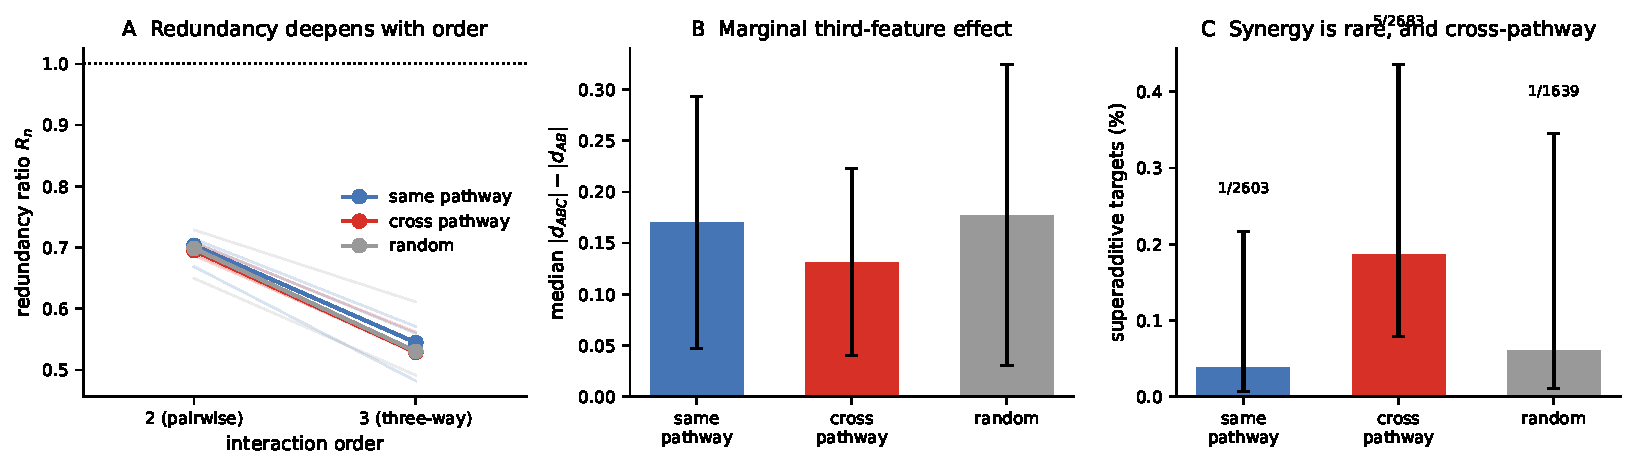
\includegraphics[width=\textwidth]{Fig3.pdf}
\caption{{\bf Redundancy deepens with interaction order; synergy is rare.} (A)~Redundancy ratio at pairwise and three-way order, per triplet, grouped by class. (B)~Marginal effect of the third feature given the first two are ablated. (C)~Fraction of target features classified superadditive ($R>1.2$), with Wilson intervals, for same-pathway, cross-pathway and random triplets.}
\label{fig:redundancy_deepens}
\end{figure}

\begin{table}[t!]
\centering
\caption{{\bf Three-way ablation by triplet class.} Redundancy ratios are medians over target features significant in at least one condition; superadditive targets satisfy $R_{ABC}>1.2$. Cross-pathway triplets are 4.9$\times$ more likely to yield a superadditive target than same-pathway triplets, but with four triplets per class the contrast is not significant (Fisher's exact $p=0.22$).}
\label{tab:threeway}
\small
\begin{tabular}{lrrrrr}
\toprule
Class & Triplets & Pairwise $R$ & 3-way $R$ & Superadditive & Rate \\
\midrule
Same-pathway & 4 & 0.703 & 0.544 & 1/2{,}603 & 0.038\% \\
Cross-pathway & 4 & 0.695 & 0.529 & 5/2{,}683 & 0.186\% \\
Random & 4 & 0.698 & 0.530 & 1/1{,}639 & 0.061\% \\
\midrule
All & 12 & 0.699 & 0.530 & 6/6{,}925 & 0.087\% \\
\bottomrule
\end{tabular}
\end{table}

\subsection{Steering: the direction of the shift is carried by the feature, not the layer}

The switch features track late pseudotime by construction, and the published state-shift metric $\Delta s$ is built from early/late pseudotime signatures. Any result stated in those terms risks circularity. We therefore expanded the panel from 14 to 80 features (12 ON-switch and 8 OFF-switch per layer, of which 75 fire in at least 10 of the 160 early-pseudotime cells), added a dose--response grid, and evaluated every intervention against three readouts that never see the pseudotime signature (Fig.~\ref{fig:steering_directionality}, Table~\ref{tab:steering}).

\paragraph{The intervention is a dose-dependent channel.}
Across the 29 features measured at five values of $\alpha$, the magnitude of the effect increases monotonically with $\alpha$ for 27/29 features on $\Delta s$, 27/29 on the marker score, 25/29 on $\Delta P(\text{terminal})$ and 25/29 on predicted pseudotime; the sign is stable across the whole dose range for 22--29 of 29 depending on the readout. Whatever these interventions are doing, they are not numerical noise.

\paragraph{OFF-switch features reverse the effect at layer 17.}
If ``layer-17 features push cells toward maturity'' were a property of the layer, or of the metric, then OFF-switch features at layer 17 would push the same way as ON-switch features. They do the opposite. At $\alpha=5$, layer-17 ON-switch features raise the held-out maturity probe in 83\% of cells (10/12 features significantly positive after Benjamini--Hochberg correction), while layer-17 OFF-switch features lower it in 88\% of cells (7/8 features significantly negative). The contrast is significant (Mann--Whitney $p=0.0055$) and is reproduced by $\Delta s$ ($p=0.039$). Directionality is carried by what the feature encodes.

\paragraph{The layer gradient is real but modest, and only two readouts see it.}
Among ON-switch features, the effect on the held-out maturity probe increases with layer depth (Spearman $\rho=+0.36$ between layer index and mean effect, $p=0.017$; layer-17 mean $+1.1\times10^{-2}$ against $+2.1\times10^{-3}$ for earlier layers). $\Delta s$ shows the same ordering more weakly ($\rho=+0.23$, $p=0.15$). The predicted-pseudotime probe does not resolve it ($\rho=+0.06$, $p=0.71$), and the literature marker panel runs against it ($\rho=-0.18$, $p=0.25$). The published claim that layer-17 features \emph{universally} drive maturation---fraction positive $=1.0$ across 3/3 features---does not survive the larger panel: with 12 layer-17 ON-switch features the mean fraction positive is $0.83$ on the maturity probe and $0.74$ on $\Delta s$.

\paragraph{The readouts disagree, and the disagreement is informative.}
$\Delta s$ and the marker-panel score are \emph{negatively} correlated across features (Spearman $\rho=-0.43$, $p=6.5\times10^{-5}$; sign agreement 36\%), while $\Delta s$ agrees only weakly with the maturity probe ($\rho=+0.17$, $p=0.14$). By contrast, $\Delta s$ computed from signatures derived from bone marrow alone, or from blood and spleen alone, reproduces the pooled $\Delta s$ almost exactly ($\rho=0.92$ and $\rho=1.00$). $\Delta s$ is thus robust to which cells define its signature and fragile with respect to what the signature means: it is a self-consistent measure of movement toward a pseudotime-derived logit profile, and it is not interchangeable with movement toward canonical maturation markers. The layer-17 ON/OFF contrast is the one conclusion that survives on both $\Delta s$ and an independent probe (Fig.~\ref{fig:steering_nonc}).


\begin{figure}[t!]
\centering
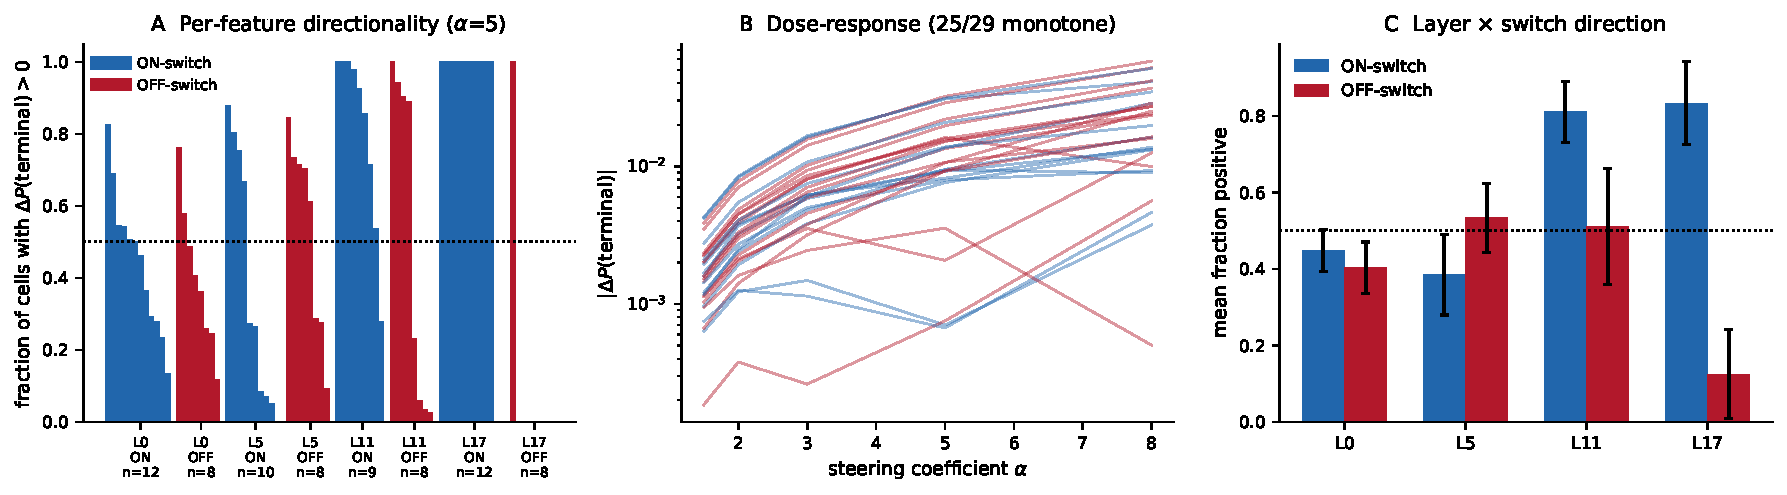
\includegraphics[width=\textwidth]{Fig4.pdf}
\caption{{\bf Steering directionality at $\alpha=5$, measured by a held-out maturity probe.} (A)~Per-feature fraction of cells with increased $P(\mathrm{terminal})$, grouped by layer and by switch direction; $n$ is the number of features surviving the 10-cell minimum. (B)~Dose--response: effect magnitude against $\alpha$ for the features measured on the full grid. (C)~Mean fraction positive by layer and switch direction (SEM). Layer-17 ON- and OFF-switch features push in opposite directions.}
\label{fig:steering_directionality}
\end{figure}

\begin{figure}[t!]
\centering
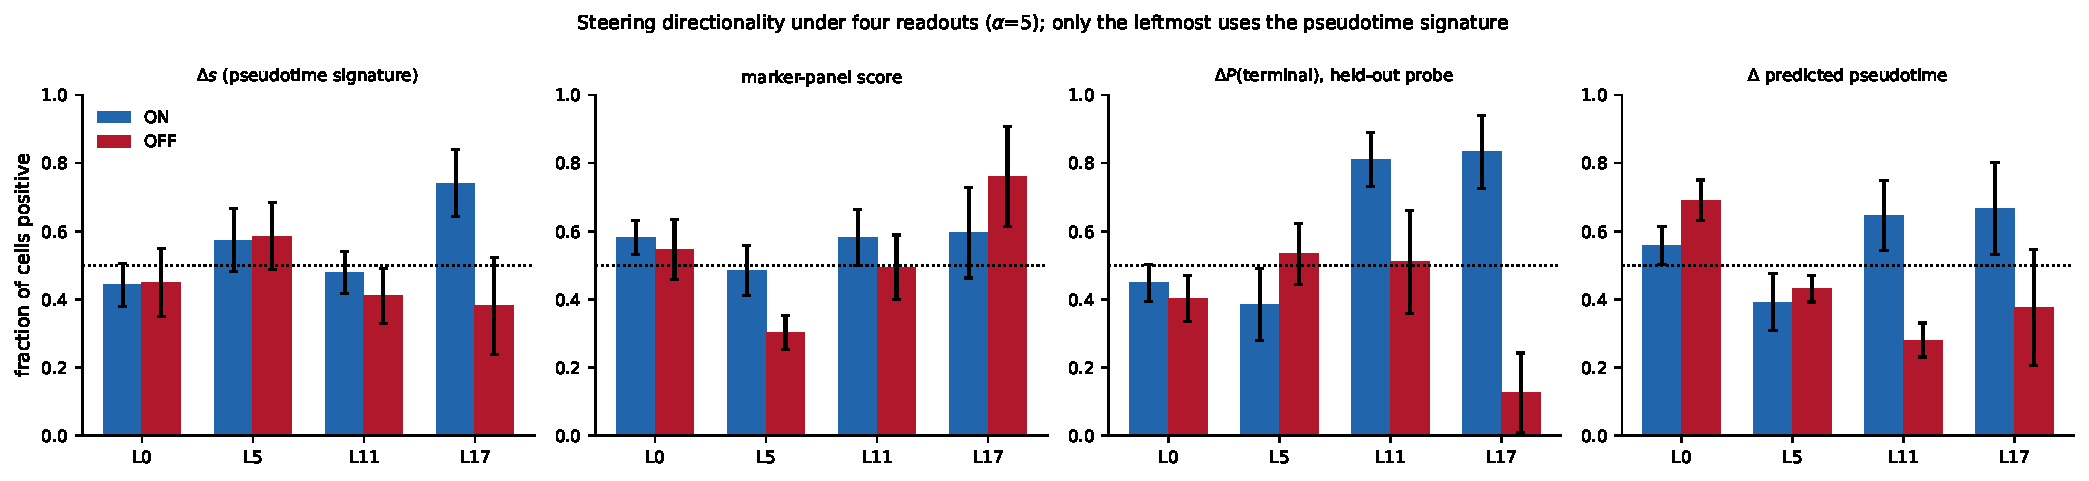
\includegraphics[width=\textwidth]{Fig5.pdf}
\caption{{\bf The same interventions under four readouts.} Fraction of cells with a positive change, by layer and switch direction, at $\alpha=5$. Only the leftmost panel ($\Delta s$) uses the pseudotime signature that also defined the feature panel; the other three are independent of it. The layer-17 ON/OFF reversal appears in $\Delta s$ and in the held-out maturity probe, but not in the literature marker panel.}
\label{fig:steering_nonc}
\end{figure}

\begin{table}[t!]
\centering
\caption{{\bf Steering panel at $\alpha=5$.} Features are grouped by source layer and switch direction. ``Feat.'' is the number surviving the 10-cell minimum (of 12 ON and 8 OFF selected per layer); ``Cells'' is the median number of early-pseudotime cells in which a feature fires. Entries are the mean across features of the per-feature fraction of cells with a positive change, under four readouts: $\Delta s$ (state shift), Marker (marker-panel score), $\Delta P$ (held-out $\Delta P(\mathrm{terminal})$ probe), and $\Delta$pt (predicted-pseudotime probe). Only $\Delta s$ uses the pseudotime signature that defined the panel.}
\label{tab:steering}
\small
\setlength{\tabcolsep}{5pt}
\begin{tabular}{llrrrrrr}
\toprule
Layer & Switch & Feat. & Cells & $\Delta s$ & Marker & $\Delta P$ & $\Delta$pt \\
\midrule
L0  & ON  & 12 & 27  & 0.44 & 0.58 & 0.45 & 0.56 \\
L0  & OFF & 8  & 110 & 0.45 & 0.55 & 0.40 & 0.69 \\
\midrule
L5  & ON  & 10 & 22  & 0.57 & 0.48 & 0.38 & 0.39 \\
L5  & OFF & 8  & 72  & 0.59 & 0.30 & 0.53 & 0.43 \\
\midrule
L11 & ON  & 9  & 26  & 0.48 & 0.58 & 0.81 & 0.65 \\
L11 & OFF & 8  & 57  & 0.41 & 0.49 & 0.51 & 0.28 \\
\midrule
L17 & ON  & 12 & 65  & 0.74 & 0.60 & \textbf{0.83} & 0.67 \\
L17 & OFF & 8  & 76  & 0.38 & 0.76 & \textbf{0.12} & 0.38 \\
\bottomrule
\end{tabular}
\end{table}

\subsection{Hub architecture survives a change of SAE training context}

The published cross-cell-line check applied K562-trained SAE features to immune cells and found weak hub-ranking agreement, but this is uninterpretable: a feature that does not fire cannot be ablated, so its degree is mechanically zero, and the comparison confounds a cell-type effect with a failure of the feature basis to transfer. We therefore repeated the trace with an SAE trained \emph{natively} on Tabula Sapiens immune activations (available at layers 0, 5, 11 and 17), tracing 400 active L5 features on 20 immune cells at downstream layers 11 and 17, and compared against the K562 trace restricted to the same two layers.

The architecture replicates; the density does not. With a native SAE the degree distribution is, if anything, \emph{more} concentrated than in K562 (Gini 0.90 versus 0.34; skewness 3.1 versus 2.2; 13.8\% of features carry more than five times the median degree, versus 0.4\%), so the heavy-tailed, hub-dominated shape is a property of the model rather than of the K562 feature basis. Annotation--centrality independence also holds: 70\% of the top-20 native hubs are unannotated and the correlation between degree and annotation is slightly negative ($\rho=-0.14$), as at the deeper K562 layers. What does not transfer is the absolute edge density---mean degree is 9.6 against 172 on the same downstream layers, and the median native feature has no significant edges---and the frequency--degree coupling is much weaker ($\rho=0.16$ versus $0.79$). Both reflect the immune population being far more transcriptionally homogeneous than proliferating K562 cells: fewer features fire, and those that do fire on a narrower range of cells, so few ablations clear the effect-size threshold. The hub architecture is thus a general property of Geneformer under an SAE decomposition; its \emph{scale} is cell-type-specific, and the earlier low rank-correlation was an activation-frequency artefact rather than evidence of a different circuit organisation.

\subsection{The circuit map does not predict CRISPRi perturbation strength}

Every intervention above is internal to Geneformer. To ask whether the recovered structure carries biological information, we tested the most direct prediction the map makes: if high-degree features are computational bottlenecks organising real transcriptional programs, the genes loading on them should be genes whose knockdown perturbs the K562 transcriptome strongly.

Using the genome-scale K562 CRISPRi screen~\citep{replogle2022mapping}, we quantified the transcriptome shift of each of 2{,}023 perturbed genes against non-targeting controls, standardised by a cell-count-matched control-resampling null, and assigned each of 2{,}384 L5 features the mean shift $z$-score of its top-50 loading genes present in the screen.

There is no association. Spearman $\rho=+0.021$ between feature degree and perturbation strength ($p=0.30$; gene-label permutation $p=0.44$), $\rho=-0.013$ after partialling out activation frequency and mean expression ($p=0.54$), and $\rho=-0.024$ using frequency-residualised degree ($p=0.24$). Hub features (top 1.8\%, $n=43$) have a mean shift $z$ of 37.0 against 35.5 for the remainder (Mann--Whitney $p=0.19$). The only significant correlate of perturbation strength in this analysis is mean expression level ($\rho=+0.087$, $p=2\times10^{-5}$), which is a property of the genes, not of the model.

This is a null result, and we report it as the boundary of what the circuit map supports. Model-internal centrality does not predict biological perturbation magnitude. Ablating an SAE coefficient and knocking down a gene are different operations, and the graph recovered by the former should not be read as a map of the latter.

\section{Discussion}
\label{sec:discussion}

\subsection{Calibration changes what an edge count means}

The single most consequential result here is not a property of Geneformer but of the method used to study it. An edge criterion stated as an effect size and a consistency fraction, applied to tens of millions of tests on twenty cells, sounds permissive and is in fact conservative---but only because most target features are unreachable and contribute exactly zero effect, and because a consistently signed effect across twenty cells is hard to produce by accident. Measured, the false-discovery rate of the published criterion is 3.6\%, and 79\% of the graph survives explicit Benjamini--Hochberg control. Neither of those facts was known before it was measured, and neither is guaranteed to hold at a looser threshold: at $|d|>0.3$ the same graph is 35.0\% noise.

Two practices follow for this literature. Edge counts obtained at different cell counts are not comparable, because the effect-size criterion becomes strictly harder to pass as $n$ grows; the ``27$\times$ more edges'' that exhaustive tracing appears to recover over selective tracing is a statement about feature coverage, not about how much circuitry either method finds. And any structural claim---hub identity, degree distribution, attenuation---should be shown to be stable across the range of thresholds where the false-discovery rate is controlled, as we do here.

\subsection{Centrality, frequency, and the limits of annotation}

Degree in this graph is largely a restatement of activation frequency ($\rho=0.84$). This is not an artefact to be corrected away: a feature that participates in the model's computation on many tokens \emph{is} more central in any reasonable sense. But it does mean that ``hub'' should not be read as ``specialised regulatory bottleneck'', and that comparisons of hub sets across layers or cell types must control for how often the features fire. It is also why the earlier hub-fragility hypothesis fails: the highest-degree features are the ones the redundant representation can most easily do without, and ablating them damages masked-gene prediction less, not more, than ablating a typical feature.

Against that background, the annotation result is narrower than previously stated and, we think, more useful. Annotation status is close to uninformative about centrality at layer 5, and the top-20 hubs there are if anything slightly \emph{more} annotated than background. What is true is that selecting features by annotation quality---the rule used by the selective circuit map---silently discards 8 of the 20 highest-degree features at L5, and 16 of 20 at L14, where hubs \emph{are} significantly annotation-depleted. The consequence for practice is the same as before: interpretability pipelines for single-cell foundation models should not pre-filter features by annotation. The reason is different: not that hubs hide in the unannotated set, but that ontologies and centrality are nearly orthogonal, and that this orthogonality worsens with depth. The parallel to study bias in network biology~\citep{szklarczyk2023string,gillis2014bias} is to the sampling process, not to the underlying network.

\subsection{Redundancy as a design principle, synergy as a rare exception}

The redundancy ratio falls monotonically from 1.0 (single) through $0.70$ (pairwise) to $0.53$ (three-way): ablating a second and a third feature from a set costs progressively less. This resonates with neural-network pruning, where large fractions of parameters can be removed without performance loss~\citep{frankle2019lottery}, and with distributed representations~\citep{hinton1986distributed,olsson2022context} in which many directions carry partly redundant copies of the same information.

What the extended panel adds is that this is not a statement about biology. Triplets whose three features share no annotated pathway are exactly as subadditive as triplets drawn from a single pathway. The earlier reading---that features within a pathway hold redundant copies of that pathway's program---is not supported: the redundancy is generic to the representation, and would have been observed for almost any three directions. Conversely, the near-absence of synergy is now bounded rather than asserted, and the one place it appears is between pathways, not within them. Conjunctive regulation across distinct signals is a common motif in biological signalling~\citep{alon2007network}; if Geneformer implements anything of the kind, our data locate it in cross-pathway feature combinations and put its prevalence below roughly $0.3\%$ of downstream targets.

\subsection{What steering does and does not show}

Amplifying a layer-17 ON-switch feature moves Geneformer's output toward the model's representation of mature cells, and amplifying a layer-17 OFF-switch feature moves it away; the effect scales with dose and is detected by a probe trained on cells the steering never touched, using ontology labels rather than pseudotime. That is an interventional result about a representation. It is not evidence that these features control differentiation in cells, and the disagreement between our readouts marks exactly where the interpretation should stop: a literature-defined marker panel, which is what a biologist would actually measure, correlates \emph{negatively} with the pseudotime-derived state-shift metric across features. A metric can be perfectly reproducible---$\Delta s$ computed from bone-marrow cells reproduces $\Delta s$ computed from blood and spleen at $\rho=0.92$---and still not measure maturation.

The layer gradient survives in weakened form: among ON-switch features the maturity probe increases with depth ($\rho=+0.36$, $p=0.017$), but ``universal'' drive at layer 17 was an artefact of testing three features. This is consistent with the progressive-refinement picture~\citep{kendiukhov2025circuits}, in which early and middle layers carry gene co-expression structure and late layers carry processed cell-identity structure, and it mirrors the biological hierarchy from multipotency maintenance to fate commitment~\citep{orkin2008hematopoiesis,graf2009forcing}. It does not establish that hierarchy causally.

\subsection{What the circuit map does not carry}

The clearest boundary comes from the one test that leaves the model. Feature degree is uncorrelated with the transcriptome-wide effect of knocking down the genes that load on that feature, in a genome-scale CRISPRi screen on the very cell line the SAE was trained on. Ablating an SAE coefficient removes a direction from a representation; CRISPRi removes a transcript from a cell. Our results say those two operations induce unrelated notions of importance. Any claim that ablation-derived circuit structure recovers regulatory structure needs to be argued against this null, not around it. It also suggests where the biology may live: not in degree, which is dominated by firing frequency, but in the identity and content of the features themselves, which is what the annotation and steering analyses probe.

\subsection{Scale of the computational graph}

The calibrated graph contains roughly $1.1$ million edges from a single source layer. With 18 layers and $\sim$4{,}000 active features each, a full map would hold tens of millions of edges, and the attenuation pattern (49.8\% of edges land at the adjacent layer, 18.4\% at the output) provides only partial compression. Two of our findings change how that scale should be read. Because degree is largely a function of activation frequency, a large fraction of those edges are contributed by a minority of frequently firing features, and any sampling scheme that ignores firing statistics will mis-estimate the graph. And because the edge criterion's false-discovery rate is a steep function of the effect-size threshold, the size of a reported circuit graph is as much a property of the threshold as of the model. Comparisons of graph size---across layers, cell types, or models---are meaningless without both controls.

\subsection{Limitations}

The exhaustive trace uses $n=20$ cells per feature, one tenth of the selective baseline; the resulting graph is more complete in features and less sensitive per feature, and the two are not interchangeable. Only three downstream layers were measured, though the attenuation shape is preserved across all 12 for the top-200 hubs (Supplementary Material). Every result is conditioned on layer~5 as the source: a single source layer samples $1/18$ of the model's depth, and although the heavy-tailed degree distribution, the frequency--degree coupling and the annotation--centrality independence replicate at L2, L8 and L14 on 500-feature subsamples, the L5 hub identities themselves do not transfer. Three-way ablation covers 12 new and 8 previously reported triplets; it can bound the superadditive rate but cannot rule out synergy in feature combinations we did not test. Steering was measured on 75 features in 160 early-pseudotime cells of one immune population, and its readouts disagree. All tracing used K562 cells and a K562-trained SAE; tracing with a natively trained Tabula Sapiens SAE reproduces the heavy-tailed architecture but at far lower edge density, so the \emph{scale} of the circuit graph is cell-type-specific even though its shape is not. Finally, every experiment used Geneformer. Whether the calibrated architecture described here holds for scGPT~\citep{cui2024scgpt} or scBERT~\citep{yang2022scbert} is untested, and given that the degree distribution is largely a shadow of the activation-frequency distribution, cross-model comparison will need to control for SAE sparsity and feature-firing statistics before any architectural difference can be attributed to the models.


\section{Conclusion}
\label{sec:conclusion}

Calibrated against an empirical null, exhaustive single-layer circuit tracing of Geneformer yields a graph that is heavy-tailed but not scale-free, dominated by features whose degree mostly reflects how often they fire, and deeply redundant: ablating a second and a third feature from a pathway costs less and less. Synergy, where it exists at all, is rare and appears between pathways rather than within them. Late-layer features steer the model's output toward its own representation of mature cells, and the direction of that shift is set by what the feature encodes rather than by the layer it sits in---but the shift does not agree with canonical maturation markers, and feature centrality carries no information about the transcriptomic consequences of knocking the corresponding genes out. Three practical conclusions follow. Interpretability pipelines for single-cell foundation models should not pre-filter features by annotation, because centrality and annotation are nearly independent. Edge counts must be calibrated and must not be compared across sample sizes. And model-internal causality, however carefully established, is not biological causality: bridging the two requires the kind of held-out biological test that, in this study, the circuit map failed.

\section{Data availability}
\label{sec:data_availability}

All analysis code, trained SAE models, and experimental results are available at \url{https://github.com/Biodyn-AI/sae-biological-map}. The repository contains \texttt{REPRODUCIBILITY.md}, which maps every script to the artefact it produces and to the table, figure or number in this paper that uses it, and lists software versions, hardware, SHA-256 hashes of all SAE checkpoints, and every random seed (cell sampling, permutation, bootstrap, triplet draw, mask positions, probe training split).

Because the exhaustive re-trace costs approximately nine GPU-hours, we deposit the intermediate products needed to reproduce every reported statistic without repeating it: the per-cell effect vectors for all 4{,}065 traced features at each downstream layer (from which every Cohen's $d$, Hedges' $g$, permutation $p$-value, false-discovery rate and threshold-sweep entry is a pure function); the calibrated edge tables; the per-cell values of all four steering readouts for every feature and every $\alpha$; the per-cell, per-condition effect vectors for all triplets; the per-perturbation CRISPRi shift $z$-scores; and the 481-cell SAE activation matrices and diffusion pseudotime that define the switch-feature panel. A validation mode (\texttt{p1a\_retrace\_with\_deltas.py --validate}) reproduces the published per-feature edge counts exactly and Cohen's $d$ to within float32 rounding.

Datasets used: K562 CRISPRi perturbation data~\citep{replogle2022mapping} at Figshare (DOI:~\url{10.6084/m9.figshare.21452470}); Tabula Sapiens~\citep{tabula2022tabula} at CZ CELLxGENE; Geneformer V2-316M~\citep{theodoris2023transfer} at \url{https://huggingface.co/ctheodoris/Geneformer}; Gene Ontology~\citep{ashburner2000go} at \url{http://geneontology.org/}.






\section*{Declaration of competing interest}
The author declares that he has no known competing financial interests or personal relationships that could have appeared to influence the work reported in this paper.

\section*{Acknowledgments}
The author thanks the developers of Geneformer, scanpy, and PyTorch. This work was self-funded by the author.

\bibliographystyle{abbrvnat}
\bibliography{references}

\end{document}
